\begin{figure}[t]
\begin{center}
%\framebox[4.0in]{$\;$}
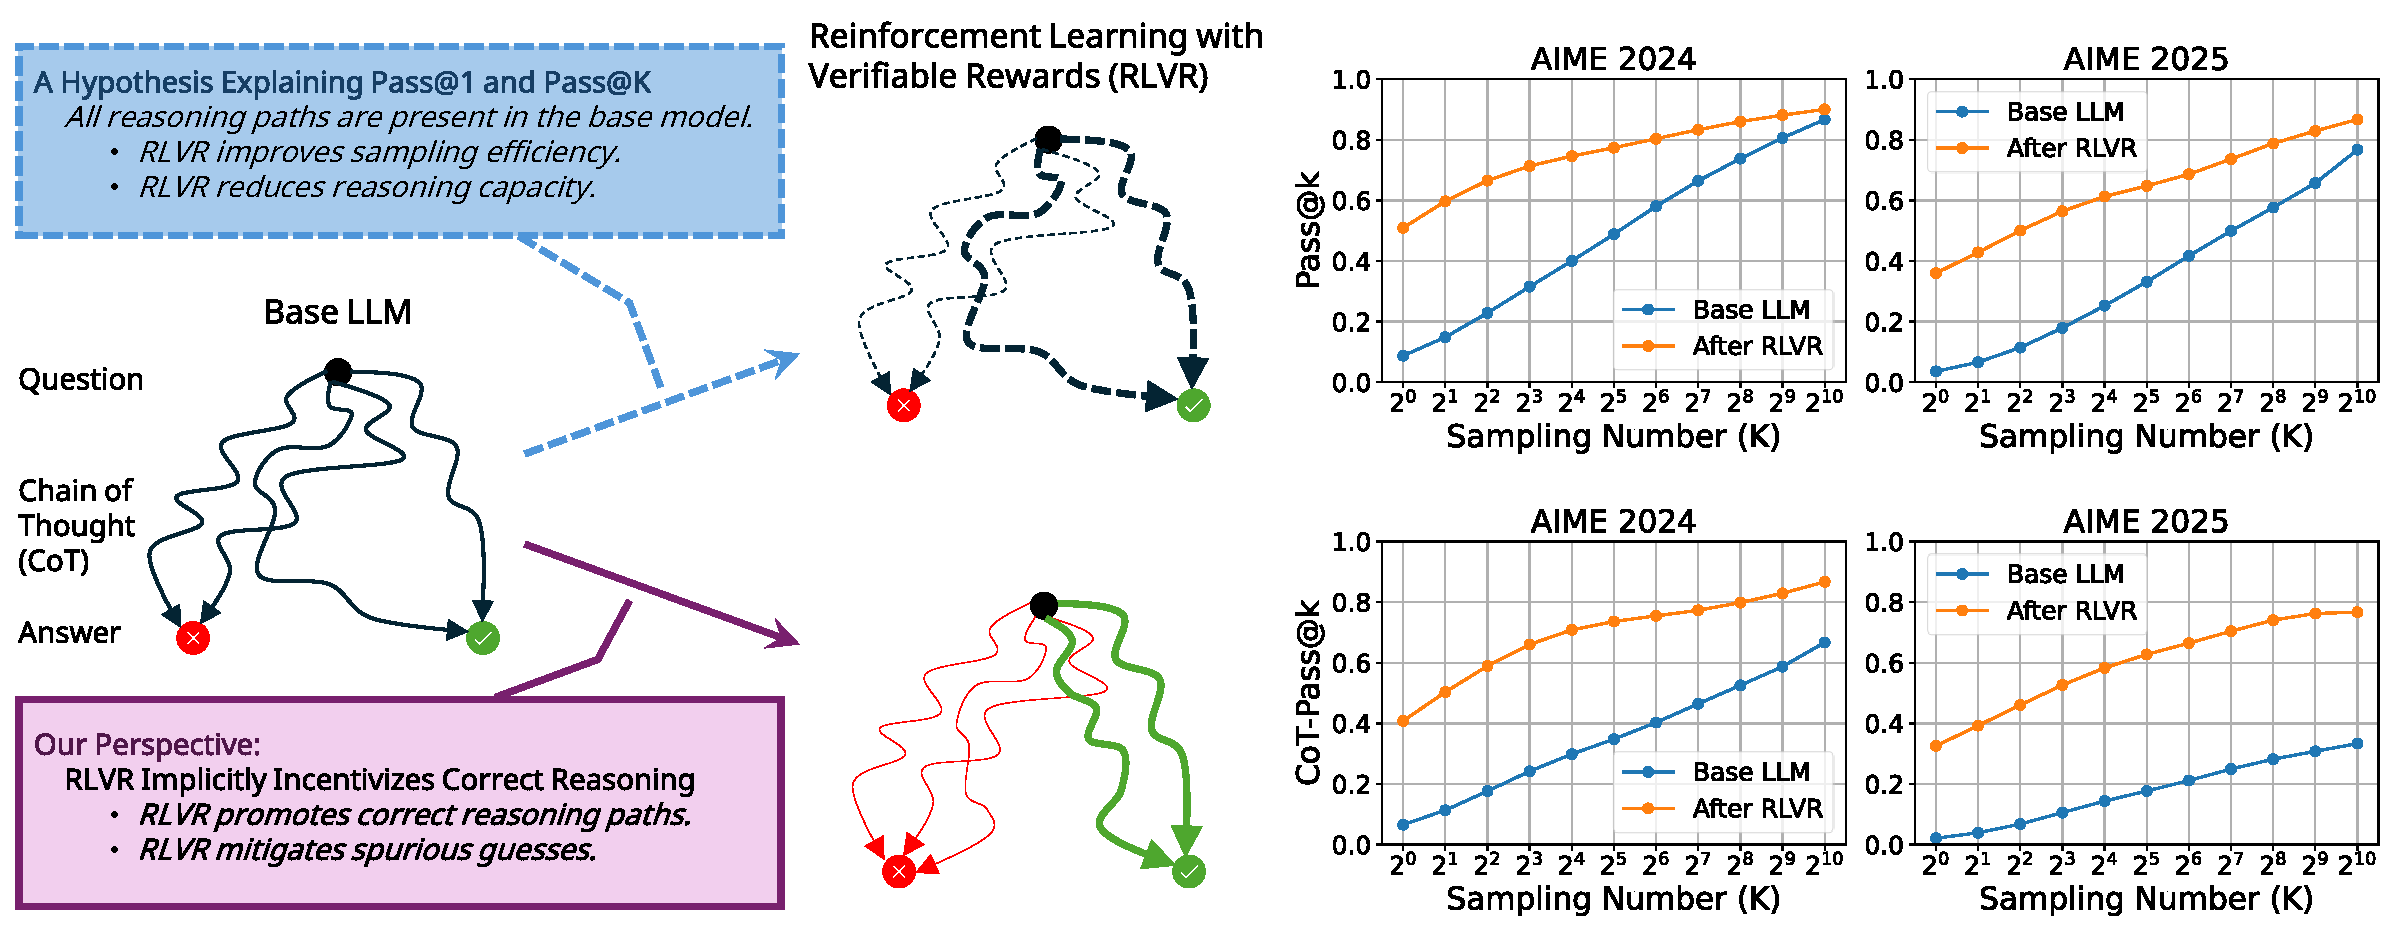
\includegraphics[width=1.0\textwidth]{figures/intro_fig.pdf}
\end{center}
\caption{
An illustration of our perspective: \textbf{RLVR implicitly incentivizes correct reasoning in base LLMs}.
We visualize how different explanation frameworks lead to varying reasoning paths being activated, with our perspective shown in the lower left and a recent popular hypothesis explaining Pass@K observations~\citep{yue2025RLVR_limit} summarized in the upper left.
In this diagram, the line width represents the sampling probability of a reasoning path, while the color distinguishes correct paths (green) from incorrect ones (red).
If all reasoning paths after applying RLVR are already present in the base model, the reasoning model merely adjusts the sampling probabilities of these existing paths (visualized in dashed lines).
This hypothesis effectively accounts for the key observation shown in the upper-right part, where, for a moderately large $K$, a base LLM can catch up to the reasoning model after RLVR using the Pass@K metric.
In this study, we unveil \textbf{the extended reasoning capability boundary} in math tasks using a refined metric, \textbf{CoT-Pass@K}, which emphasizes both the correctness of answers and the validity of reasoning CoTs.
}
\label{fig:first_fig}
\end{figure}


\section{Introduction}
\label{sec:intro}

The successful replication of long chain-of-thought (CoT) reasoning, similar to that in OpenAI's o1~\citep{openai2024o1}, by DeepSeek-R1~\citep{guo2025deepseek-r1} using the Group Relative Policy Optimization (GRPO) algorithm~\citep{shao2024deepseekmath}, has sparked a surge of interest within the open research community. This interest is focused on understanding, reproducing, and extending DeepSeek's approach, as evidenced by a multitude of recent studies~\citep{liu2025DrGRPO-Oat-Zero,hu2025OpenReasonerZero,zeng2025SimpleRL-Zoo-Zero,yu2025DAPO-Zero,he2025Skywork-OR1,wen2025Light-R1,chen2025AceReason-Nemotron}. Fundamentally, this emerging paradigm is a form of Reinforcement Learning with Verifiable Rewards (RLVR)~\citep{lambert2024Tulu3,guo2025deepseek-r1,yue2025RLVR_limit}, where a Large Language Model (LLM) acts as a policy, generating a CoT as a sequence of actions and receiving feedback on answer correctness from deterministic verifiers. This paradigm holds the promise of endowing LLMs with the ability to learn from experience through free exploration, potentially leading to unlimited intelligence~\citep{openai2024o1,guo2025deepseek-r1,silver2025EraOfExp}.

However, emerging concerns question the true effectiveness of RLVR. These concerns are motivated by the observation that some post-RLVR models improve the Pass@1 metric but fail to enhance the Pass@K metric compared to the base (pre-RLVR) model. This phenomenon was first noted by~\cite{shao2024deepseekmath} during the development of GRPO. Subsequently, a systematic study by~\cite{yue2025RLVR_limit} on more open-weight RLVR models discovered that the Pass@K metric of the base model increases at a much faster rate than its RLVR-tuned counterpart. Consequently, for a moderately large K, the base model eventually matches and surpasses the reasoning model. This led to their adventurous hypothesis: all correct reasoning paths are already present in the base model, and RLVR merely improves sampling efficiency at the cost of reducing overall reasoning capacity.

While this hypothesis has gained significant support~\citep{zhu2025PosNegRLVR,zhang2025EMPO,wang2025MultimodalCoTRM,chen2025NFT}, conflicting observations have also been reported. For instance,~\cite{liu2025ProRL} detected the emergence of new reasoning patterns after RLVR, while they also acknowledged a loss in reasoning capacity as measured by Pass@K.~\cite{chen2025AceReason-Nemotron} reported persistent improvements in Pass@K for competitive coding tasks but did not show improved Pass@K for math tasks.~\cite{Shojaee2025IllusionOfThink} observed similar Pass@K observations on math datasets but found different patterns on puzzles with high complexity.
To the best of our knowledge, no systematic explanation exists to reconcile these contradictory findings, leaving a critical question unanswered: ``\emph{should we accept the hypothesis as a fundamental limitation of RLVR or should we trust new empirical findings that challenge the hypothesis?}''

In this work, we address this debate systematically and demonstrate that RLVR can fundamentally enhance the reasoning abilities of LLMs.
First, we revisit Pass@K experiments and unveil the existence of extended reasoning capability boundaries after RLVR for both math and code tasks.  
In addition to reproducing the extended reasoning boundary in competitive coding, as reported by~\citet{chen2025AceReason-Nemotron}, we find that the Pass@K performance of base LLMs on math reasoning can be unreliable, as base LLMs are capable of producing incorrect CoTs yet coincidentally arriving at the ground truth, especially for hard mathematical questions where answers are simple and can be easily guessed after multiple attempts.
To address this, we introduce a new metric, CoT-Pass@K, which evaluates success only when both the final answer and the intermediate reasoning CoT are correct.  
In practice, we verify the correctness of mathematical CoTs by instructing DeepSeek-R1-0528-Qwen3-8B~\citep{deepseek2025R1-0528} and confirm their reliability.
Using this new metric, we successfully identify the extended reasoning boundary of a post-RLVR model for math tasks.  
Figure~\ref{fig:first_fig} summarizes our key perspectives.


Moreover, we develop a theoretical framework to explain why RLVR works, even when base LLMs may guess the ground truth and only answer correctness is provided as a reward, and how RLVR incentivizes correct reasoning. Our central insight is that once LLMs have been pre-trained to establish strong knowledge and logic priors that distinguish correct from incorrect CoTs, the GRPO gradient will increase the probability of generating more correct CoTs.

Additionally, we investigate the training dynamics of RLVR to understand when this improved reasoning emerges. By reproducing GRPO-style training using the open-source DAPO recipe~\citep{yu2025DAPO-Zero} and performing extensive verifications, we find that RLVR begins to incentivize correct reasoning from the early stages of training, and this capability generalizes well to unseen test questions. The results of our training analysis align with our theorem, which highlights the implicit incentivization of correct reasoning CoTs.

Finally, we evaluate the quality of generated CoTs from a learning perspective: if supervised learning on some CoT data results in better generalization performance on test sets, we regard them as high quality. This allows us to evaluate the quality of CoTs generated by model checkpoints at different RLVR stages. Our results show that after RLVR, the quality of reasoning CoTs has been fundamentally improved.

In summary, our contributions include:
\begin{itemize}
    \item A systematic evaluation revealing the extended reasoning capability boundary after RLVR for both code and math tasks.
    \item A theoretical understanding of why RLVR works with only answer correctness as a reward and how RLVR incentivizes correct reasoning.
    \item An analysis of RLVR's training dynamics, delving deeper into optimization effects, generalization behaviors, and current limitations.
    \item Confirmation of the quality improvements in reasoning CoTs from a learning perspective, replicating the generalization abilities of post-RLVR models trained with enormous costs simply via supervised fine-tuning.
\end{itemize}

